\documentclass[11pt, oneside]{article}      % use "amsart" instead of "article" for AMSLaTeX format
\usepackage{geometry}                       % See geometry.pdf to learn the layout options. There are lots.
\geometry{letterpaper}                          % ... or a4paper or a5paper or ... 
%\geometry{landscape}                       % Activate for rotated page geometry
%\usepackage[parfill]{parskip}          % Activate to begin paragraphs with an empty line rather than an indent
\usepackage{graphicx}               % Use pdf, png, jpg, or eps§ with pdflatex; use eps in DVI mode
                      % TeX will automatically convert eps --> pdf in pdflatex        
\usepackage{amsmath,amsthm,amssymb}
\usepackage{mathtools}
\usepackage{xcolor}
\usepackage[font=small,labelfont=bf,skip=0pt,justification=justified]{caption}
\usepackage{tikzit}
\input{zx.tikzdefs}
\input{zx.tikzstyles}
\usepackage{hyperref} % must be last package used

\setlength{\parindent}{0in}

% Commands

\newcommand{\bra}[1]{\ensuremath{\left\langle #1 \right|}}
\newcommand{\ket}[1]{\ensuremath{\left|  #1 \right\rangle}}
\newcommand{\braket}[2]{\ensuremath{\langle#1|#2\rangle}}
\newcommand{\ketbra}[2]{\ensuremath{\ket{#1}\!\bra{#2}}}

\theoremstyle{definition}
\newtheorem{theorem}{Theorem}[section]
\newtheorem{corollary}[theorem]{Corollary}
\newtheorem{lemma}[theorem]{Lemma}
\newtheorem*{lemma*}{Lemma}
\newtheorem*{proposition*}{Proposition}
\newtheorem{proposition}[theorem]{Proposition}
\newtheorem{conjecture}[theorem]{Conjecture}
\newtheorem{definition}[theorem]{Definition}
\newtheorem{example}[theorem]{Example}
\newtheorem{remark}[theorem]{Remark}

\title{\textbf{Efficiently Calculating Jones Polynomials at Lattice Roots of Unity with the ZX Calculus (Draft)}}
\author{
  Alex Townsend-Teague
  \and
  Konstantinos Meichandzitis
}
\date{}

\begin{document}
\maketitle

\section{Introduction}

[Use Konstantinos' O.G. notes from the start of this project, and introduce the qubit and qutrit ZX calculi]\newline

For the case $q=3$ we use the qutrit ZX calculus:
\begin{equation}
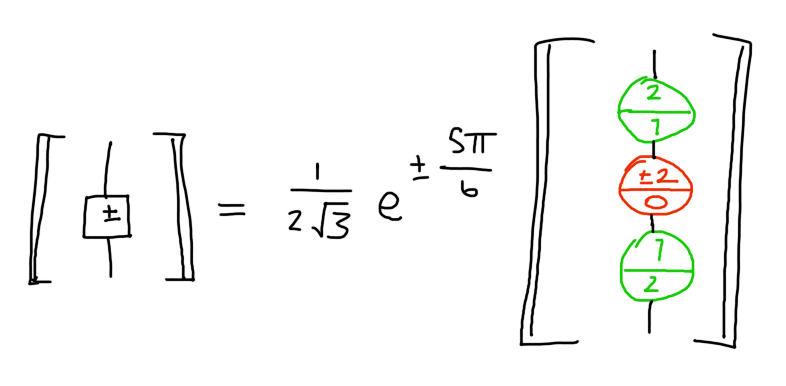
\includegraphics[scale=0.3]{Images/Qutrit Potts matrices.png}
\end{equation}

For the case $q=4$ we are back again in the usual qubit ZX calculus:
\begin{equation}
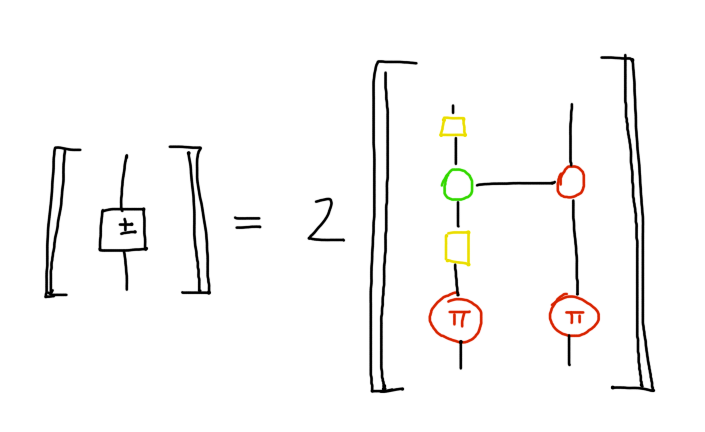
\includegraphics[scale=0.3]{Images/Qu(4)it Potts matrices.png}
\end{equation}

In each case, the resulting map is in the stabilizer fragment of the ZX calculus. 

\section{Simplifying Qubit ZX Diagrams}

In [cite Aleks' paper] the authors give an efficient algorithm for reducing any qubit stabilizer ZX diagram to one of vastly smaller size [specific bound?]. In our case, since any knot will be transformed by the process above into a ZX diagram with zero inputs and zero outputs, this gives an efficient algorithm for reducing the diagram to a scalar.\newline

[Summarise Aleks' algorithm]\newline

This suffices to prove our main result for the cases $q \in \{2, 4\}$. However, it doesn't yet give us a useful algorithm for explicitly calculating Jones polynomials, because throughout the method above equality is considered only up to a complex scalar multiple. Therefore we now give a scalar-exact version.\newline

[Give scalar-exact version]\newline

\section{Simplifying Qutrit ZX Diagrams}

For the remaining case $q=3$, we will show that we can generalise all the ideas of the previous section to the qutrit ZX calculus.

\subsection{Graph-Like Qutrit ZX Diagrams}

% \numbered{Definition}{A \textit{Hadamard edge} (or \textit{H-edge}) is a Hadamard map connecting two spiders. A \textit{Hadamard adjoint edge} (or \textit{$H^\dagger$-edge) }}

[Make all of the following scalar-exact]\newline

We first define a graph-like diagram in the qutrit ZX calculus.

% \numbered{Definition}{A qutrit ZX diagram is \textit{graph-like} when:}
\begin{definition}\label{def:graph_like_qutrit}
A qutrit ZX diagram is \textit{graph-like} when: 
\begin{enumerate}
	\item Every spider is a Z-spider.
	\item Spiders are only connected by Hadamard edges ($H$-edges) or their adjoints ($H^\dagger$-edges).
	\item Every pair of spiders is connected by at most one $H$-edge or $H^\dagger$-edge.
	\item Every input and output is connected to a spider.
	\item Every spider is connected to at most one input or output.
\end{enumerate}
\end{definition}

Note the difference compared to the qubit case: we need not worry about self-loops beacuse the qutrit ZX calculus doesn't define a 'plain' cap or cup. But this comes at a cost: spiders in the qutrit case fuse more fussily. Specifically, when two spiders of the same colour are connected by at least one plain edge and at least one $H$- or $H^\dagger$-edge, fusion is not possible. The following equation, which holds with the roles of $H$ and $H^\dagger$ reversed, helps us get around this:

\begin{equation}\label{eq:spiders_reluctant_to_fuse}
	\tikzfig{spiders_reluctant_to_fuse} 
\end{equation}

We will shortly show that every qutrit ZX diagram is equivalent to a graph-like one, making use of the following lemmas:

\begin{lemma}\label{lem:H_edges_qutrit} 
	The following two equations hold in the qutrit ZX calculus. Moreover, they hold with the roles of $H$ and $H^\dagger$ interchanged:
	\begin{equation}
		\tikzfig{2_hadamard_edges_become_adjoint}
		\hspace{75pt}
		\tikzfig{hadamard_edge_and_adjoint_edge_permute}
	\end{equation}
	\begin{proof}
		This is Lemma 3.4 in [cite Harny's local complementation paper].
	\end{proof}
\end{lemma}

As we will formalise later, the lemma above says we can think of Hadamard edges as single edges and their adjoints as double edges, then work modulo $3$, since every triple of parallel edges disappears.

\begin{lemma}\label{lem:H_boxes_qutrit} 
	The following three equations hold in the qutrit ZX calculus. Moreover, they hold with the roles of $H$ and $H^\dagger$ interchanged:
	\begin{equation}
		\tikzfig{4_hadamards_cancel}
		\hspace{75pt}
		\tikzfig{3_hadamards_flip}
		\hspace{75pt}
		\tikzfig{2_hadamards_separate}
	\end{equation}
	\begin{proof}
	\end{proof}
\end{lemma}

Again intuitively we can think of Hadamard boxes of having value $1$ and their adjoints $-1$ and then work modulo $4$.

\begin{corollary}\label{prop:every_diagram_is_graph_like_qutrit}
	Every qutrit ZX diagram is equivalent to one that is graph-like.
	\begin{proof}
		First use the colour change rule to turn all X-spiders into Z-spiders. Then use Lemma~\ref{lem:H_boxes_qutrit} to remove excess $H$- and $H^\dagger$-boxes, inserting a spider between any remaining consecutive pair of such boxes, so that all spiders are connected only by plain edges, $H$-edges or $H^\dagger$-edges. Fuse together as many as possible, and apply Equation~\ref{eq:spiders_reluctant_to_fuse} where fusion is not possible, so that no plain edge connects two spiders. Apply Lemma~\ref{lem:H_edges_qutrit} to all connected pairs of spiders until at most one $H$- or $H^\dagger$-edge remains between them. Finally, to ensure every input and output is connected to a spider and every spider is connected to at most one input or output, we can again add a few spiders, $H$- and $H^\dagger$-boxes as needed: 
		\begin{equation}
			\tikzfig{plain_input_output_wire_is_graph-like}
			\hspace{75pt}
			\tikzfig{input_connected_to_hadamard_is_graph-like}
			\hspace{75pt}
			\tikzfig{multiple_inputs_connected_to_one_spider_is_graph-like}
		\end{equation}
	\end{proof}
\end{corollary}

\begin{definition}\label{def:graph_state_qutrit}
	A graph-like qutrit ZX diagram is a \textit{graph state} when every spider has zero phase (top and bottom) and is connected to an output. 
\end{definition}

A graph state is described fully by its underlying multigraph, or equivalently by an adjacency matrix, where edges take weights in $\mathbb{Z}_3$ [reference Harny]. Nodes correspond to phaseless green spiders, edges of weight $1$ correspond to Hadamard edges, and edges of weight $2$ correspond to $H^\dagger$ edges. As in the qubit case, graph states admit a local complementation operation [Harny's completeness paper, Definition 2.6], though the effect is now slightly more complicated. We'll give the intuition after the formal definition:

% In this setting, a neighbour of a node is one connected to it by an edge of weight $1$ or $2$. Informally, the local complementation by $a \in \mathbb{Z_3}$ at node $k$ adds $a$ to the weight of every (perhaps zero-weighted) edge $ij$ for all neighbours $i$ and $j$ of $k$. That is, it unions with the original graph $a$ copies of the complete graph on $k$'s neighbours. Stated formally:

\begin{definition}\label{def:local_complementation_qutrit}
	Given $a \in \mathbb{Z}_3$ and a graph state $\ket{G}$ with adjacency matrix $W = (w_{i,j})$, the \textit{($a$)-local complentation} at node $k$ is the new graph state $\ket{G *_a i}$, whose adjacency matrix $W' = (w'_{i,j})$ given by:
	\begin{equation}
		w'_{i,j} = w_{i,j} + aw_{i,k}w_{j,k}
	\end{equation}
\end{definition}

So only those edges between neighbours of node $k$ are affected, but rather than just having their weight increased by $1$ (modulo $2$) as in the qubit case, the increase in weight also depends on the weights of the edges from $i$ and $j$ to $k$. As always, this is best seen graphically. We reintroduce the blue dashed line notation for Hadamard edges, and now also use purple dashed lines for $H^\dagger$-edges:

\begin{equation}
	\tikzfig{blue_dashed_line_definition}
	\hspace{75pt}
	\tikzfig{purple_dashed_line_definition}
\end{equation} 

So now for two nodes $i$ and $j$ both connected to $k$ by the same colour edge, $a$-local complementation at $k$ increases weight $w_{i,j}$ by $a$. If instead $i$ and $j$ are connected to $k$ by edges of different colour, $a$-local complementation at $k$ decreases $w_{i,j}$ by $a$:

\begin{equation}
	\tikzfig{a_local_comp_same}
	\hspace{75pt}
	\tikzfig{a_local_comp_different}
\end{equation}

Just as in the qubit case, composing local complementations gives a local pivot operation:

\begin{definition}\label{def:local_pivot_qutrit}
	Given $a,b,c \in \mathbb{Z}_3$ and a graph state $\ket{G}$, the \textit{$(a,b,c)$-local pivot} at nodes $i$ and $j$ is the new graph state $\ket{G \wedge_{(a,b,c)} ij} \defeq \ket{((G *_a i) *_b j) *_c i}$ 
\end{definition}


\end{document} 